%%%%%%%%%%%%%%%%%%%%%%%%%%%%%%%%%%%%%%%%%%%%%%%%%%%%%%%
\section{Sensors and Simulation}
\subsection{Further Sensors}

\begin{frame} 
 \frametitle{Kinect}
\begin{itemize}
 \item Motion sensing input device by Microsoft for the Xbox 360 video game console
 \item Range camera technology by Israeli developer PrimeSense
 \item 3D scene information from a continuously-projected infrared structured light
\end{itemize}
\hspace{35ex}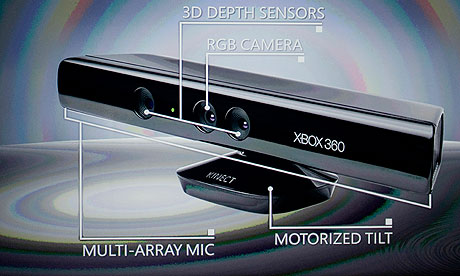
\includegraphics[width=5cm]{images/kinect.png}
\end{frame}

\begin{frame}
 \frametitle{Kinect Operations - I}

\begin{itemize}
  \item The IR camera and the IR projector form a stereo pair with a baseline of approximately 7.5\,cm
  \item The IR projector sends out a fixed pattern of light and dark speckles
  \item The pattern is generated from a set of diffraction gratings, with special care to lessening the effect of zero-order propagation of a center bright dot
\end{itemize}
\hspace{35ex}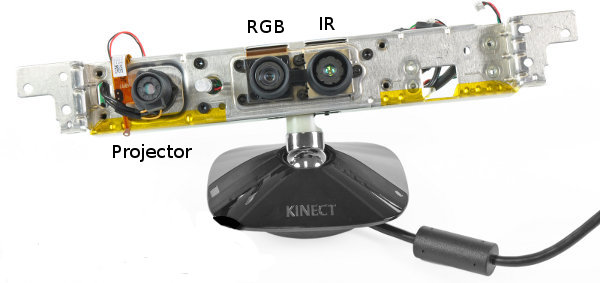
\includegraphics[width=5cm]{images/kinect2.png} 
\end{frame}

\begin{frame}
 \frametitle{Kinect - Technical Data}
\begin{itemize}
  \item Resolution of (640 $\times$ 480) @ 30 Hz (color) and (320 $\times$ 240) @ 30 Hz (depth)
  \item Angular field of view of $57^0$ horizontally and $43^0$ vertically
  \item Range of approximately 0.7 - 6\,m (practical 0.7 - 3.5\,m)
  \item Physical tilt range ($-31^0$  to $+31^0$ )
  \item Voice microphone and array supporting single speaker voice recognition (16-bit audio @ 16 kHz)
  \item OpenNI and Freenect drivers
\end{itemize}

\end{frame}


\begin{frame} 
 \frametitle{Kinect - First Results}
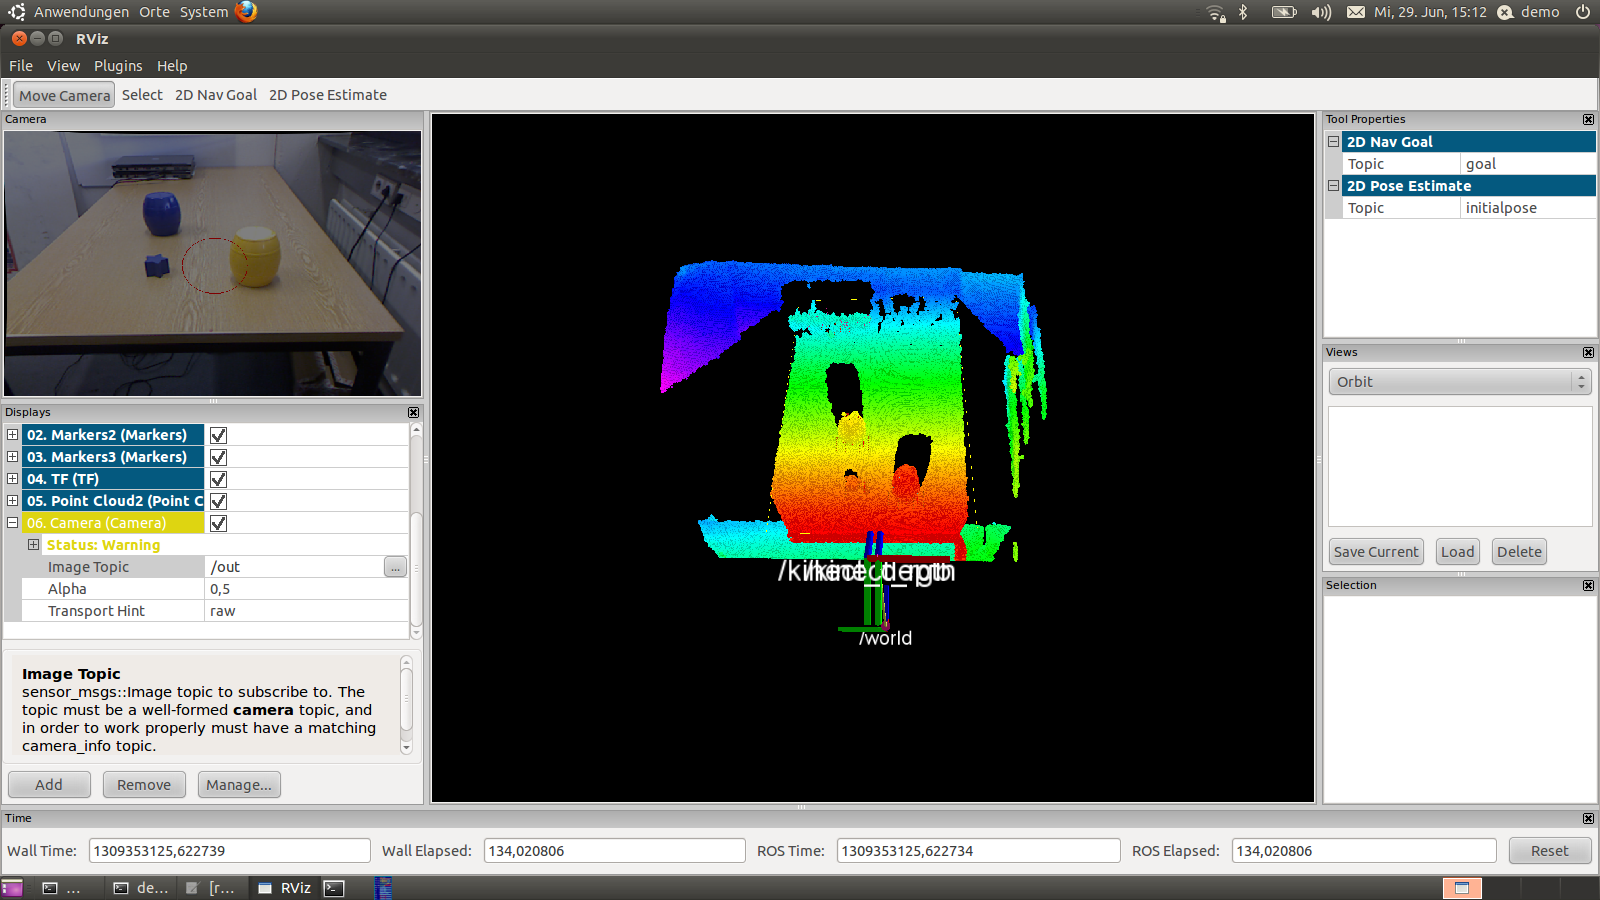
\includegraphics[width=11cm]{images/ros_rviz.png}
\end{frame}


\begin{frame}
 \frametitle{Kinect - Summary}
\begin{itemize}
  \item Fast sensor with large resolution
  \item Stable, repeatable results
  \item Ideal for surfaces, inaccuracy on edges (remedy through fusion with the tof-camera (200 $\times$ 200 @ 40 fps) or other sensors)
\end{itemize}
\hspace{3ex}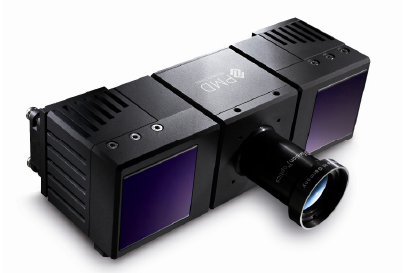
\includegraphics[width=5.5cm]{images/camcube.png}
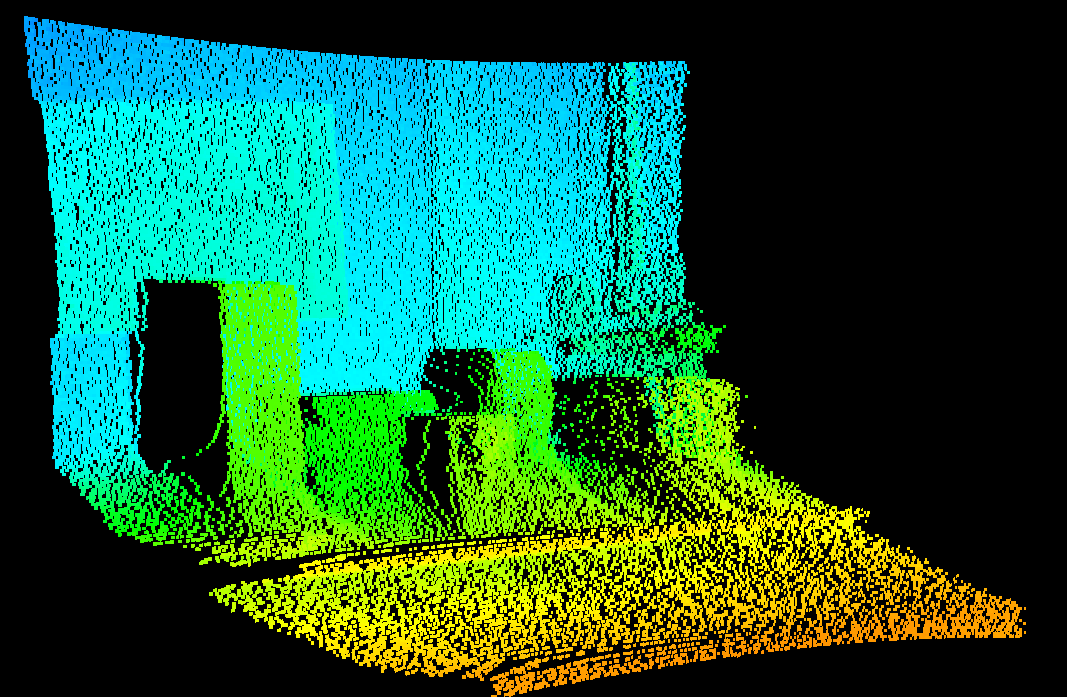
\includegraphics[width=5.5cm]{images/pmd2.png}
\end{frame}

\begin{frame}
 \frametitle{PMD Camcube in ROS}
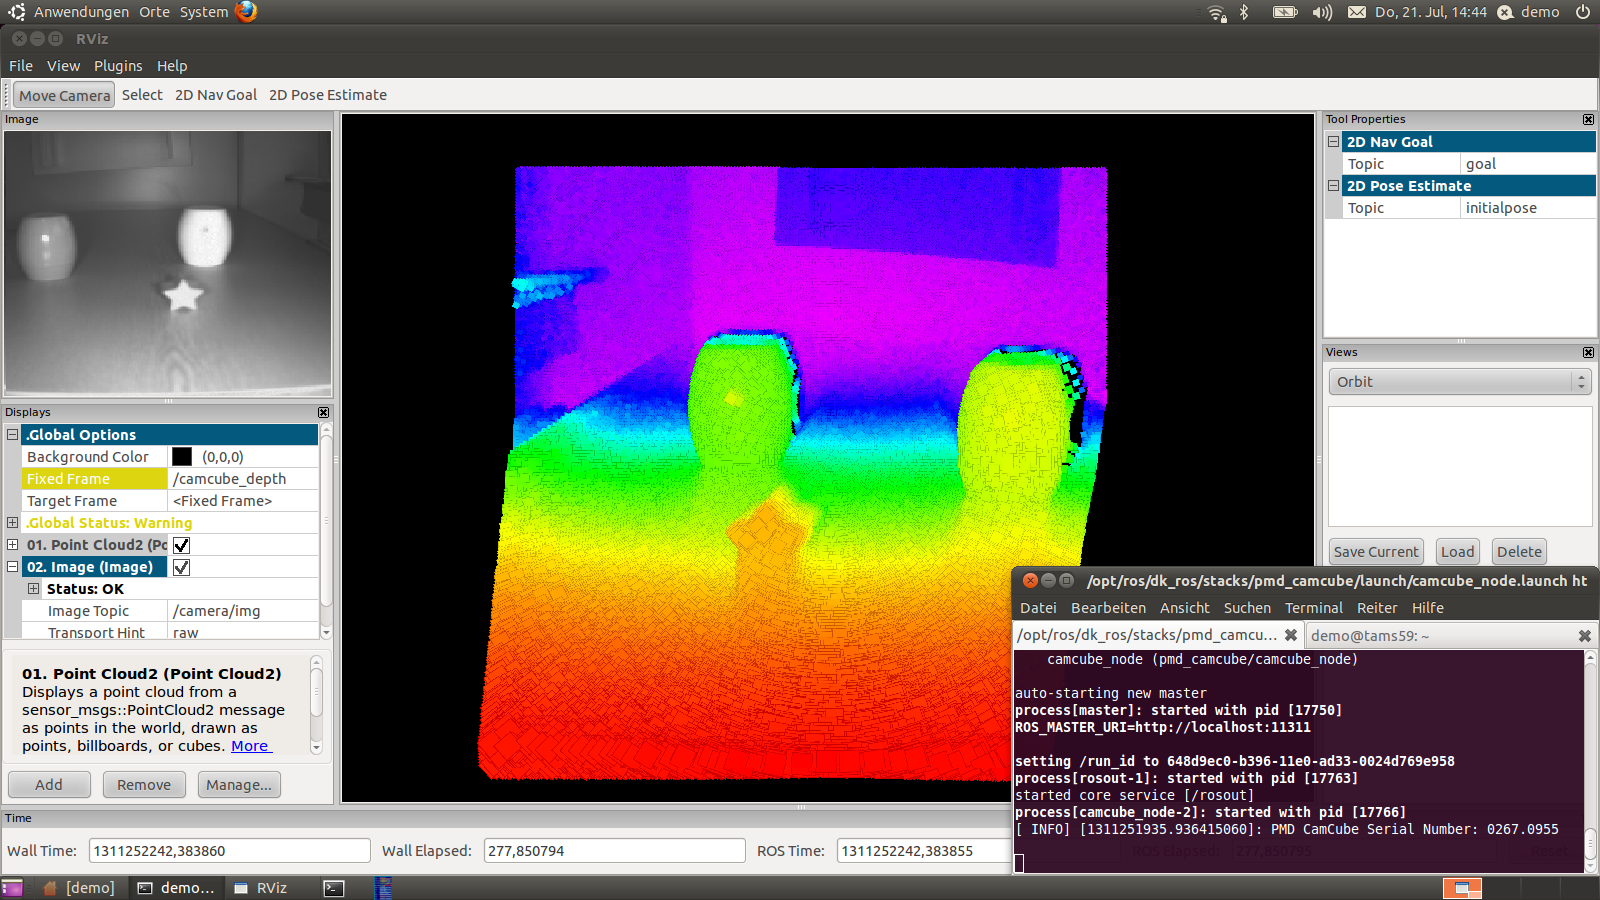
\includegraphics[width=11cm]{images/camcube_ros.png}
\end{frame}

\begin{frame}
 \frametitle{FLIR A615}
\begin{itemize}
  \item FOV $25^0 \times 19^0$
  \item IR resolution $[640 \times 480]@50$ Hz
  \item Accuracy $\pm 2^0\,C$ or $\pm 2\%$ of reading
  \item Image and control over Gigabit Ethernet
\end{itemize}

\vspace{5ex}\hspace{37ex}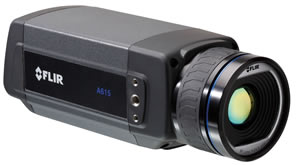
\includegraphics[width=4cm]{images/A615_300.jpg}
\end{frame}

\begin{frame}
 \frametitle{FLIR A615}
\vspace{-1ex}{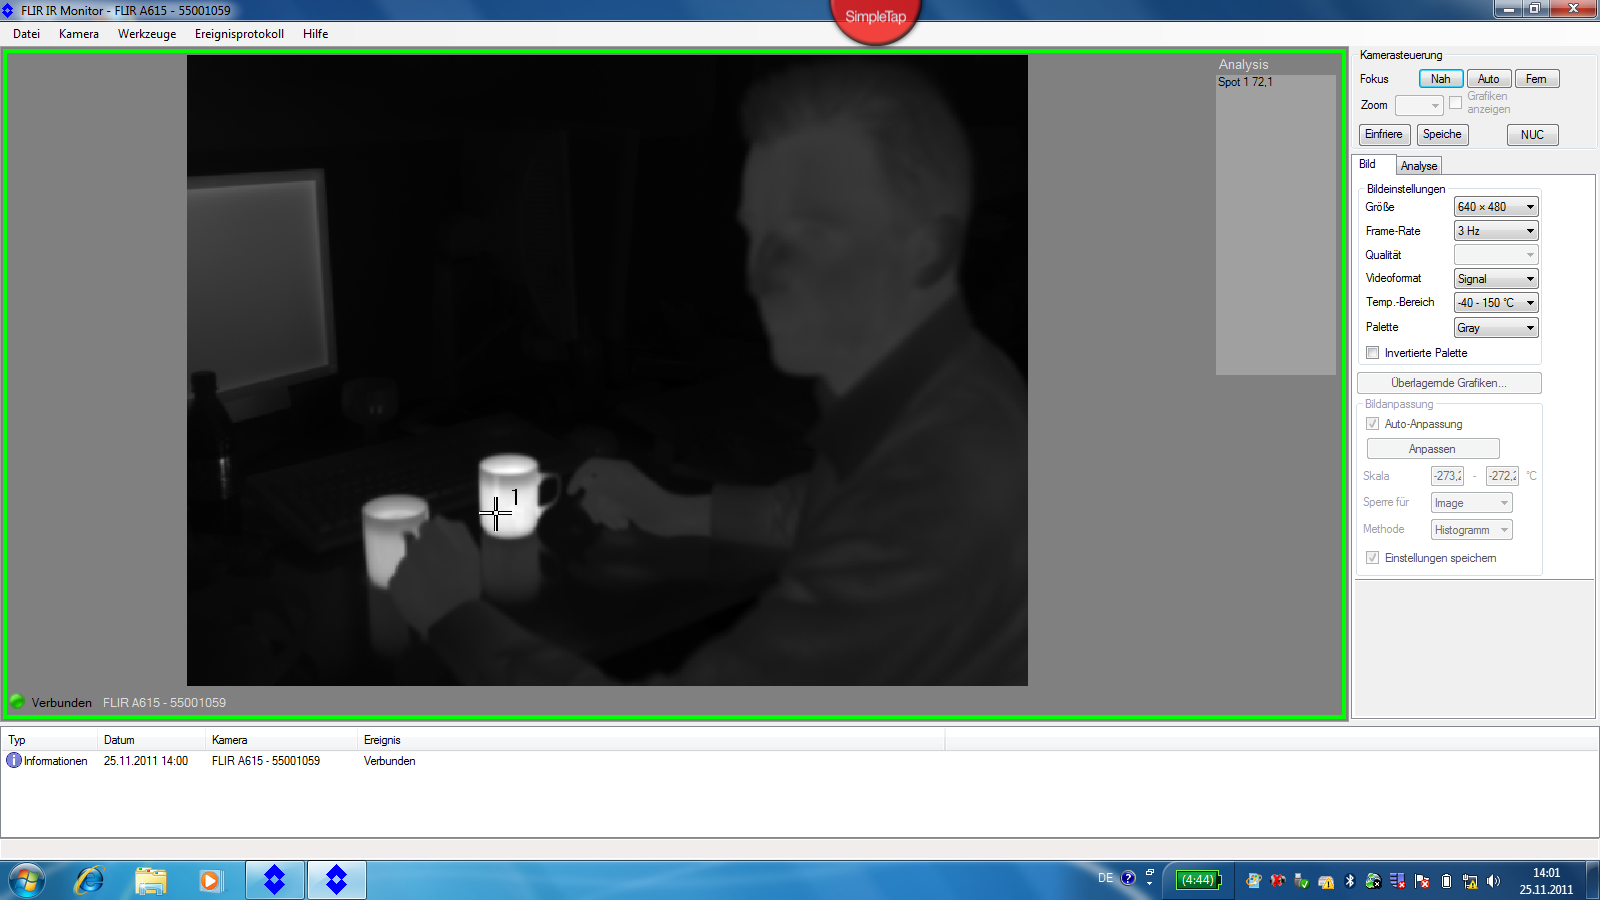
\includegraphics[width=7cm]{images/hannes_flir.png} \\
\vspace{-7ex} \hspace{22ex}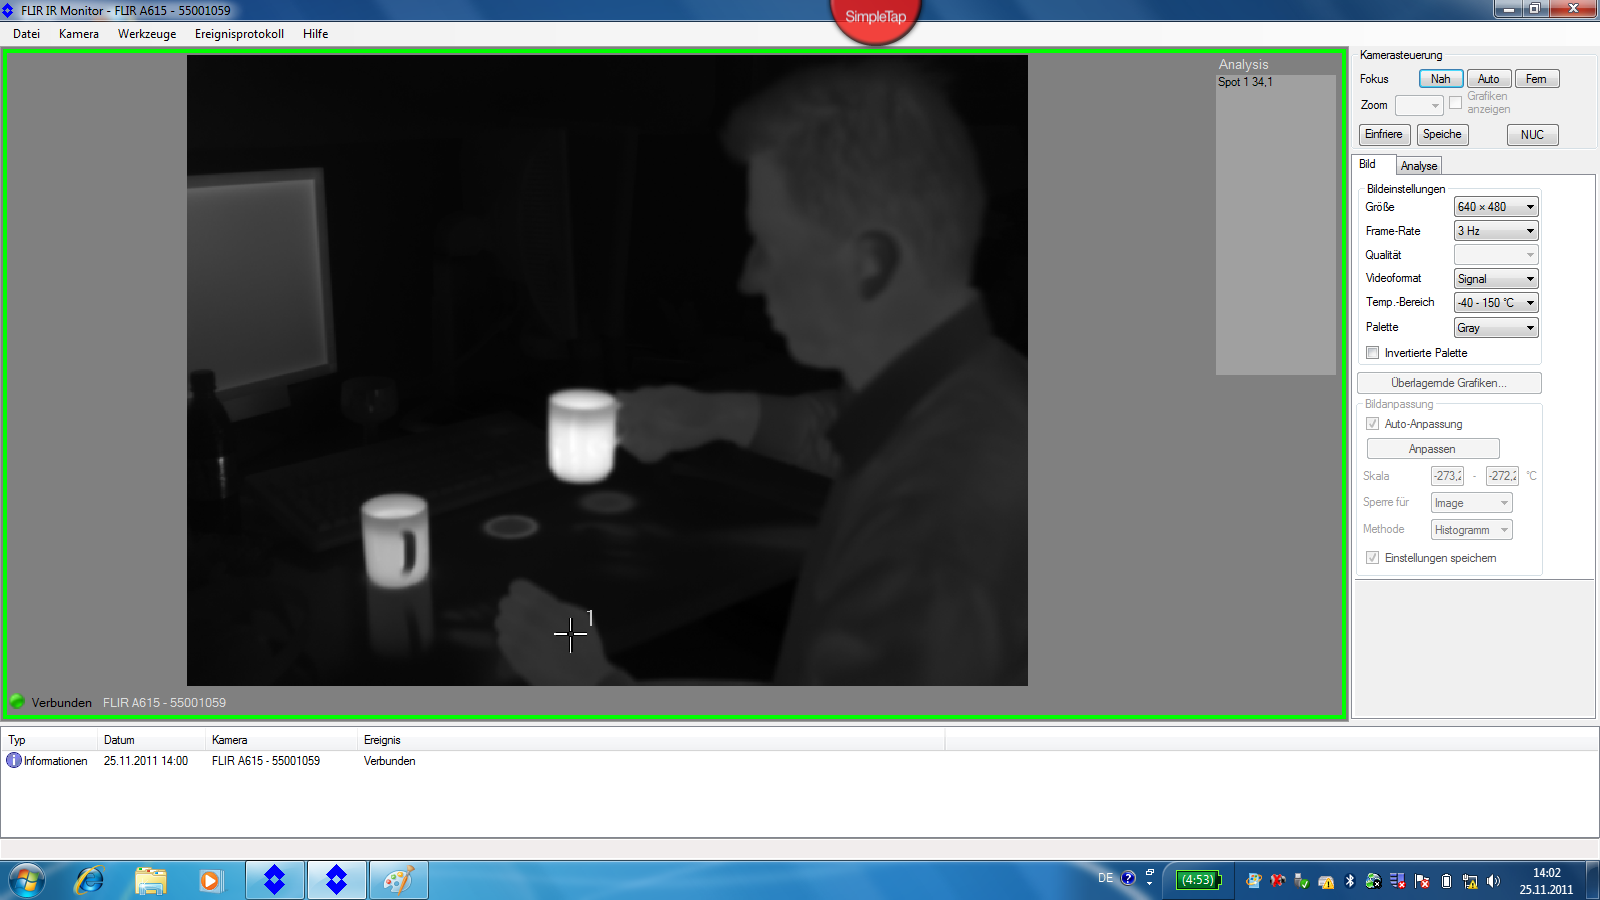
\includegraphics[width=7cm]{images/hannes_flir2.png}
}
\end{frame}

\subsection{Gazebo} % - 3D dynamic multi-robot simulation
% intro / abstract etc.			--------------------------------------
\begin{frame}
  \frametitle{Gazebo}
\begin{itemize}
    \item Developed to be fully compatible with the Player\footnote{The Player/Stage Projekt, http://playerstage.sourceforge.net/} device server
    \item Full integrated in ROS (version 1.0)
    \item 3D dynamic multi-robot simulation
    \item Open source
    \item ODE -  Open Dynamics Engine (Bullet)

   
\end{itemize}
\end{frame}

\begin{frame}
  \frametitle{Gazebo}
\begin{itemize}
    \item The World represents the set of all models and environmental factors such as gravity and lighting
    \item Accuracy in terms of robot sensors and actuators
    \item API for easily create new robots, actuators, sensors, and arbitrary objects
    \item Possibilities to create complex worlds
    \item Simulation of remote environments
    \item GUI for data visualization
    \item Visualization with help of OpenGL and GLUT
    
\end{itemize}
\end{frame}

\begin{frame}
  \frametitle{General Structure of Gazebo components}
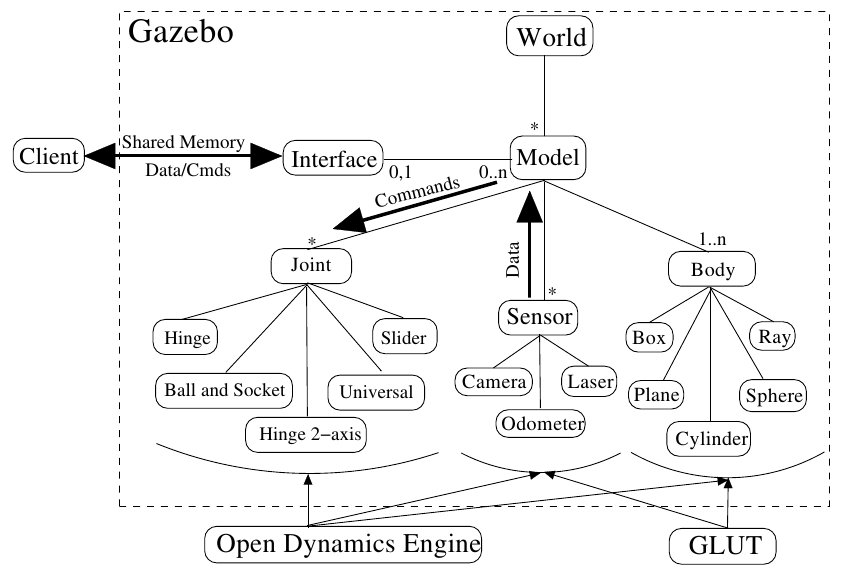
\includegraphics[width=9cm]{images/gazebo_struktur.png}
\end{frame}

\begin{frame}
  %\frametitle{}
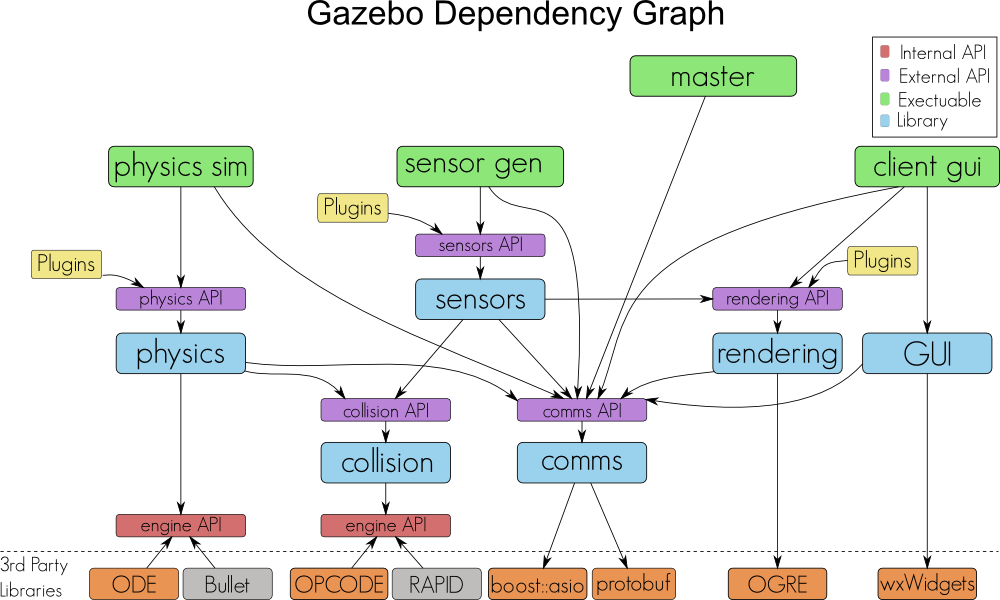
\includegraphics[width=11cm]{images/gazebo_dependency_graph.png}
\end{frame}

\begin{frame}
  \frametitle{ROS Simulation Interface}
\hspace{5ex}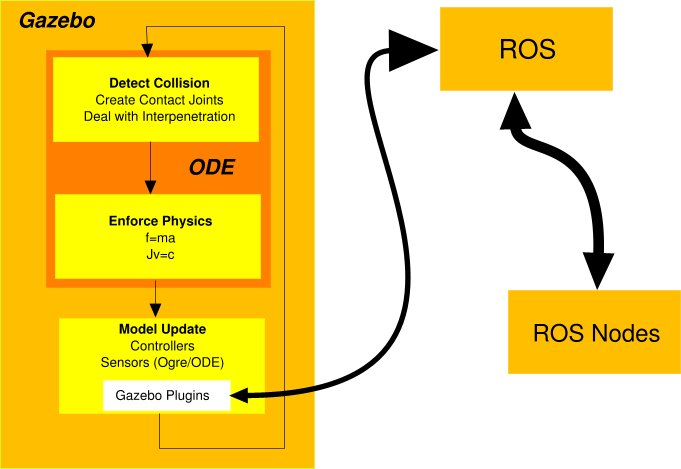
\includegraphics[width=9cm]{images/ros_simulation_interface.jpg}
\end{frame}

\begin{frame}
  \frametitle{ROS, Stage, PR2}
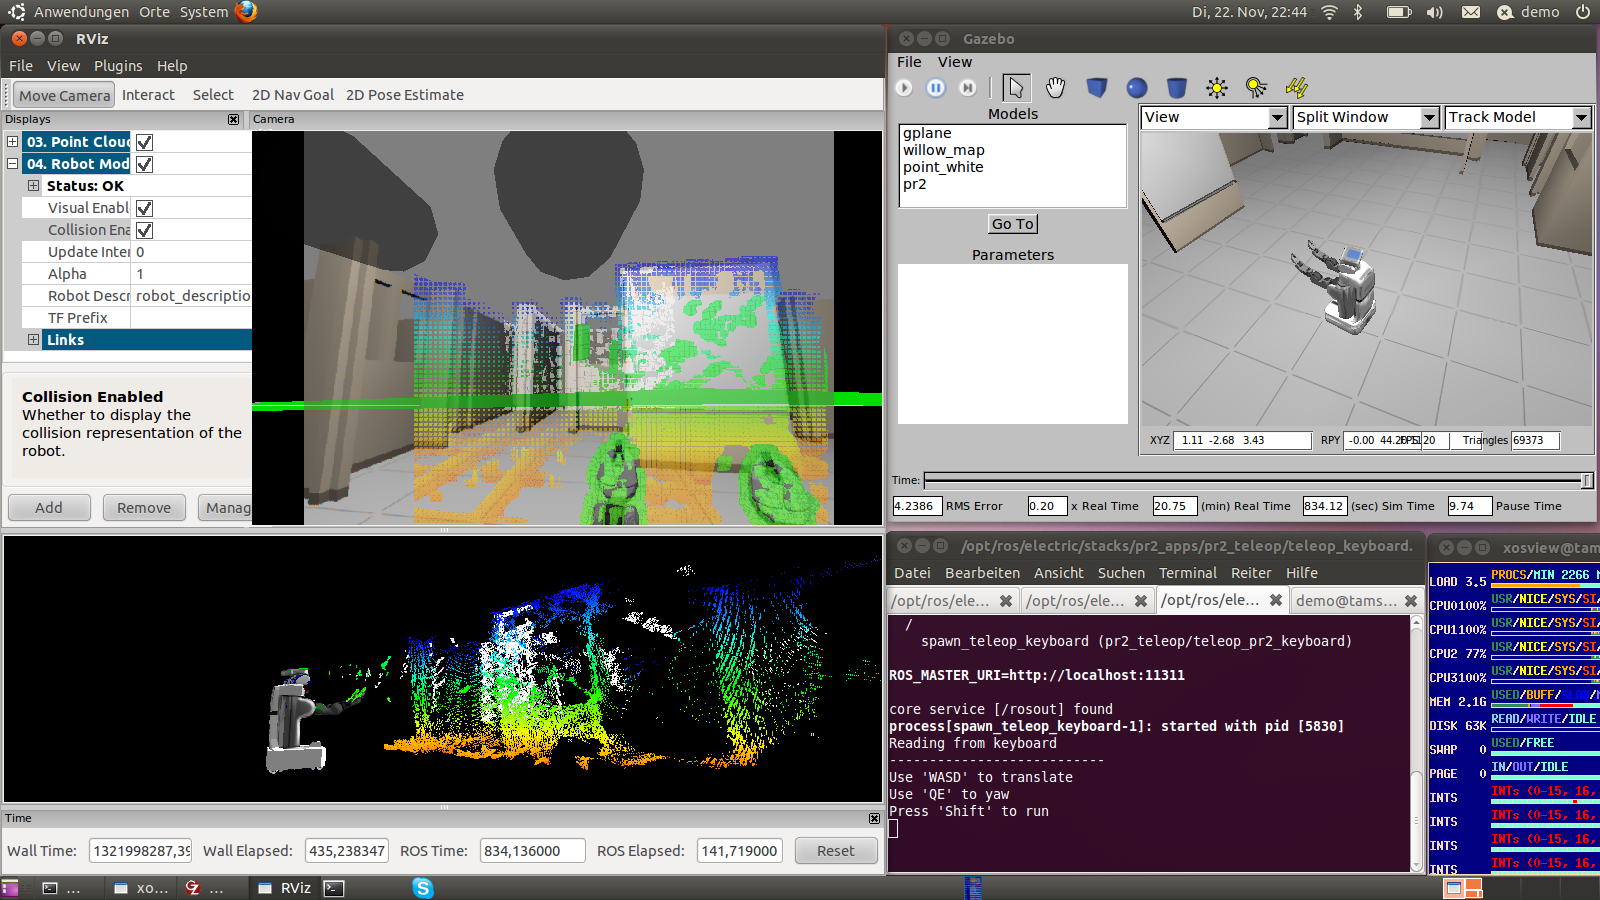
\includegraphics[width=11cm]{images/race_pr2_ros_rviz2.png}
\end{frame}
%%%%%%%%%%%%%%%%%%%%%%%%%%%%%%%%%%%%%%%%%%%%%%%%%%%%%%%
